\documentclass[12pt, a4paper]{article}
%\usepackage{natbib}
\usepackage{cite}
\usepackage{amsmath,amssymb,amsfonts}
\usepackage{algorithmic}
\usepackage{graphicx}
\usepackage{textcomp}
\usepackage{xcolor}
\usepackage[inkscapeformat=pdf]{svg}
\usepackage[inline]{enumitem}
\usepackage[hidelinks]{hyperref}

\usepackage{myacronyms}
\usepackage{listings}
\usepackage{todonotes}
\newcommand{\note}[3]{\todo[inline,linecolor=#1,backgroundcolor=#1!25,bordercolor=#1]{\textbf{#2:} #3}}
\newcommand{\angela}[1]{\note{blue}{Angela}{#1}}

\newenvironment{inlinelist}{\begin{enumerate*}[label=\emph{(\roman*)}]}{\end{enumerate*}}

\usepackage{cleveref}

\begin{document}

\title{Towards collective operating systems through Aggregate Computing}

\author{Angela Cortecchia}
\date{\today}
\maketitle


% ----------------------------------------
\section{State of the art}
\label{sec:state-of-the-art}

\sloppypar
\paragraph{Collective Adaptive Systems and Macroprogramming.}
\ac{cas} are systems composed of multiple autonomous entities,
including devices, sensors, and actuators, which interact locally to achieve a shared global objective~\cite{ferscha2015}.
%
\ac{cas} are designed to adapt to dynamic changes in the environment, system requirements, or operational conditions.
%These systems are designed to adapt to dynamic changes in the environment, system requirements, or operational conditions.
%
\ac{cas} are commonly employed in \ac{cps} applications where devices collaborate to monitor and control a
physical environment or to provide services to users.

Managing a single device in a distributed system presents several challenges,
such as \textbf{scalability}, \textbf{device heterogeneity},
\textbf{resource constraints}, and the need to adapt to \textbf{dynamic changes}.
%
Transitioning from a \emph{device-centric} approach,
where the collective is not the abstraction target,
to an \emph{aggregate-centric} approach can lead to various advantages, like
\begin{inlinelist}
    \item distributed intelligence,
    \item resource pooling,
    \item adaptability, and
    \item robustness.
\end{inlinelist}
%
The mentioned challenges can be addressed by using \emph{macroprogramming}.

\emph{Macroprogramming}~\cite{casadei2023} refers
to expressing the macroscopic behavior of a system through a single program using
macro-level abstractions.
%
This approach captures system-level behavior while abstracting individual component interactions.
%
Macroprogramming has been used in different contexts like \ac{wsn}~\cite{1440891}, \ac{iot} applications~\cite{noor19,mizzi18} and swarm robotics~\cite{buzz}.

\sloppypar
\paragraph{Self-organization and Field Calculus.}

Coordination models propose that interaction among multiple independent and autonomous software systems can be designed
orthogonally to pure computation, conceptualized as a shared data space.
%
Over time,
various approaches like \textit{Linda}~\cite{ViroliCoordination2012} and \textit{MARS}~\cite{mars} have emerged,
focusing on centralized local components rather than system distribution.
%
The primary challenges in distributed systems are adapting to environmental changes, coordinating many agents effectively, and maintaining resilience.
%
Addressing these demands a \emph{self-organizing and coordinating} approach, regulating interactions to ensure robust global coordination behavior.

%To facilitate self-organization in complex environments, the \emph{coordination field} concept was introduced as a
%navigational tool for agents.

%The tuple-based middleware \textit{TOTA} (Tuples On The Air)~\cite{tota} supports field-based coordination in pervasive
%computing applications.

%Studies on distributed intelligent systems proposed computational fields for managing space-time
%computing models, promoting higher abstractions of spatial collective adaptive systems~\cite{JLAMP2019}.

The coordination field concept aids self-organization in complex environments.
\emph{TOTA} (Tuples On The Air), a tuple-based middleware~\cite{tota}, 
supports field-based coordination in pervasive computing. 
%
Research on distributed intelligent systems has proposed computational fields for managing space-time computing models, 
promoting higher abstractions of spatial collective adaptive systems~\cite{JLAMP2019}.

\ac{fc}~\cite{TOCL2019} is a foundational model for coordinating computational devices in physical environments.
%
It captures the essentials of computational fields,
including functions over and with fields,
their temporal evolution,
and the construction of field values from neighboring devices.
%
\ac{fc} specifies system behavior through a dynamic network of directly communicating devices,
using functional compositions of operators to manipulate computational fields.
%
Local specifications involve asynchronous computational rounds with three phases:
\begin{inlinelist}
    \item \emph{context building},
    \item \emph{program execution}, and
    \item \emph{export sharing}.
\end{inlinelist}
%
Globally,
\ac{fc} aligns individual device behavior with the network's overarching behavior,
specifying mappings for each device's computation round at space-time events.

\sloppypar
\paragraph{Aggregate Computing/Programming.}
\ac{ap} (or \ac{ac})~\cite{CASADEI2019252} is a functional macroprogramming approach for the compositional development
of self-adaptive \ac{iot} services,
based on the abstractions of \ac{fc}~\cite{MAMEIZL04}.

\ac{ac} programs the behavior of distributed systems by defining interactions among devices as a whole,
shifting the computation unit from individual devices to collaborative groups.
%
This approach supports the specification, analysis, simulation,
and runtime execution of collective services across diverse IoT architectures~\cite{FI2020-pulverization}.
%
The paradigm embodies three key traits:
\begin{inlinelist}
    \item \emph{global stance with global-to-local mapping}, targeting the entire distributed IoT ecosystem,
    \item \emph{service compositionality}, describing rich collective services through functional composition, and
    \item \emph{abstraction}, enabling adaptivity by abstracting from low-level details.
\end{inlinelist}
%
These traits facilitate concise articulation of complex solutions in the design phase and provide flexibility in execution and deployment strategies during operation.
%
Each device locally evaluates the program at a set frequency and communicates with neighboring devices as needed.

\sloppypar
\paragraph{Aggregate Processes.}
\label{par:aggregate-processes}

A system has been developed to manage \emph{aggregate processes}~\cite{aggregate-processes} based on \ac{fc}
to address the challenges of managing multiple concurrent aggregate operations in a distributed environment.

Aggregate processes are concurrent field computations sustained by a dynamic team of devices,
with their spatial region opportunistically changing over time.
%
This concept captures aggregate behavior, dynamicity, context orientation, and intrinsic resiliency.
%
It offers benefits such as limiting computational resource consumption, maintaining quality of service,
and enhancing distributed computation dynamics.
%
While similar to concentrated processes,
aggregate processes allow multiple computations to overlap in both space and time,
they currently do not consider issues related to permissions, signals, or interprocess communication.

\sloppypar
\paragraph{Tools for Aggregate Computing.}
Various tools have been developed to support the \ac{ac} paradigm,
each tailored to specific characteristics and target devices.

\emph{ScaFi (Scala Fields)}~\cite{scafi} is a Scala-based framework providing a \ac{dsl}, libraries,
a simulation environment with a GUI integrated with the Alchemist simulator~\cite{PianiniJOS2013},
and an actor-based runtime for aggregate computing systems.
%
ScaFi runs aggregate programs on the \ac{jvm} and in web browsers through the ScaFi Web tool~\cite{Coordination2021-scafiweb}, for rapid prototyping.

\emph{Protelis}~\cite{PianiniSAC2015} is a functional programming language implementing a higher-order version of \ac{fc},
with a C-like syntax for building reusable components of aggregate systems.
%
It provides domain-specific APIs interoperable with Java through Protelis-Lang~\cite{SASO2017-protelislang}, but requires a \ac{jvm} to run.

\emph{FCPP}~\cite{DBLP:journals/scp/AudritoT24} is a C++ library implementing FC for simulations of distributed systems.
%
It supports running aggregate programs on low computational capacity devices but has a less ergonomic syntax.

\emph{Collektive} is a prototype \ac{dsl} extending \ac{fc} with \ac{xc}~\cite{AudritoCDSV24},
offering a more expressive language with a user-friendly syntax compared to FCPP and Protelis.
%
It is natively multi-platform, allowing development on various devices.

\sloppypar
\paragraph{Distributed Operating Systems.}
A \ac{dos}~\cite{dos} coordinates and manages resources across independent networked computational nodes,
each holding a specific subset of the global operating system.
%
It presents a unified system to the user,
akin to a centralized \ac{os}, ensuring transparency, reliability, and efficiency despite resource distribution complexity.
%
%The kernel at each node provides essential services such as process and memory management.
%
Architecturally,
a \ac{dos} must balance individual and overall system goals,
requiring a design approach that separates policy from mechanism.
%
Its functioning relies on multi-level collaboration among system components,
each node has \emph{part} of the distributed resources, and the system distributes the different processes to execute among the nodes,
while the user perceives the system as a single entity.

\subsection{Coherence with my previous experiences}
\label{subsec:coherence-with-the-educational-path}
The proposed research project extends my Master’s degree final year and thesis activities.
%
During my Master’s studies, exploration of  \ac{fc} and \ac{ac} began in the “Pervasive Computing” course.
%
My project's colleagues and I developed a Rust-based reimplementation of aggregate computing's core engine,
alongside a Scala 3 version, providing a solid foundation in \ac{fc} and \ac{ac}.

My Master’s thesis focused on expanding the Collektive DSL by integrating constructs from the \ac{xc} calculus,
demonstrating its potential for \ac{ac} applications through a prototype tested on simple case studies.

During the development of the Master's degree,
I had the opportunity to apply for a research grant that was awarded to me from the \emph{Consortium GARR}~\footnote{\url{https://www.garr.it/it/}},
the Italian ``Group for Research Networks Harmonisation'',
ongoing work extends the Collektive DSL by creating a standard library of functions for \ac{ac} application development and showcasing language functionalities through demos.

These experiences facilitated collaborations with various researchers, including a collaboration with Professor Sven Tomforde from
the University of Kiel,
on managing communication between maritime autonomous surface ships.

Furthermore,
the work done has allowed me to paper submissions to the \emph{IEEE International Conference on Autonomic Computing and Self-Organizing Systems} (ACSOS 2024),
and the \emph{International Symposium on Distributed Simulation and Real Time Applications} (DS-RT 2024),
focusing on generalizing the \emph{Vascular Morphogenesis Controller} (VMC)~\cite{ZahadatHS17} algorithm using the \ac{ac} paradigm
and developing an architecture and prototype for monitoring distributed simulations of distributed systems using Collektive.

% ----------------------------------------
\section{Project description}
\label{sec:project-description}

%\sloppypar
\subsection{Motivation.}
\label{subsec:motivation.}

Typical applications of aggregate computing implement and execute a single, albeit complex, algorithm.
%
However,
there are scenarios where these aggregated algorithms need to be added, removed,
or manipulated at runtime without affecting the others.
%
For example,
in a crowd management situation where people are directed to move in a certain direction,
congestion might occur,
requiring law enforcement to alter the movement of a portion of the crowd.

This concept parallels how modern \acp{os} manage processes, but in space and time.
%
To achieve similar functionalities in the realm of aggregate computing,
it is necessary to advance towards the development of \emph{\ac{cos}}.
%
These systems, in fact,
face concerns akin to those of ``concentrated'' \ac{os},
such as the management of devices, users, groups and relative permissions, and signals;
but in a distributed environment in which these concepts assume a different meaning
entailing space and time.
%
Additionally,
\acp{cas} are usually composed of heterogeneous devices,
meaning that the system must be able to,
simultaneously,
abstract away their differences and manage their specificities.

\subsection{Idea}
\label{subsec:idea}

\begin{figure}
    \centering
    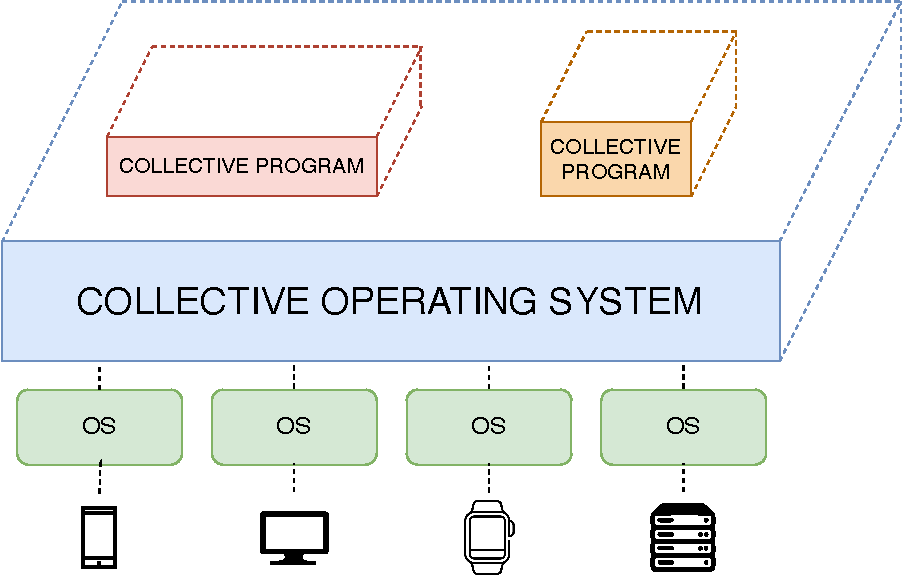
\includegraphics[width=0.8\textwidth]{figures/system}
    \caption{
        High-level view of the system.
        The collective operating system is seen as a middleware that manages the different aggregate programs and the devices
        of different types.
    }\label{fig:system}
\end{figure}

\begin{figure}[h!]
    \centering
    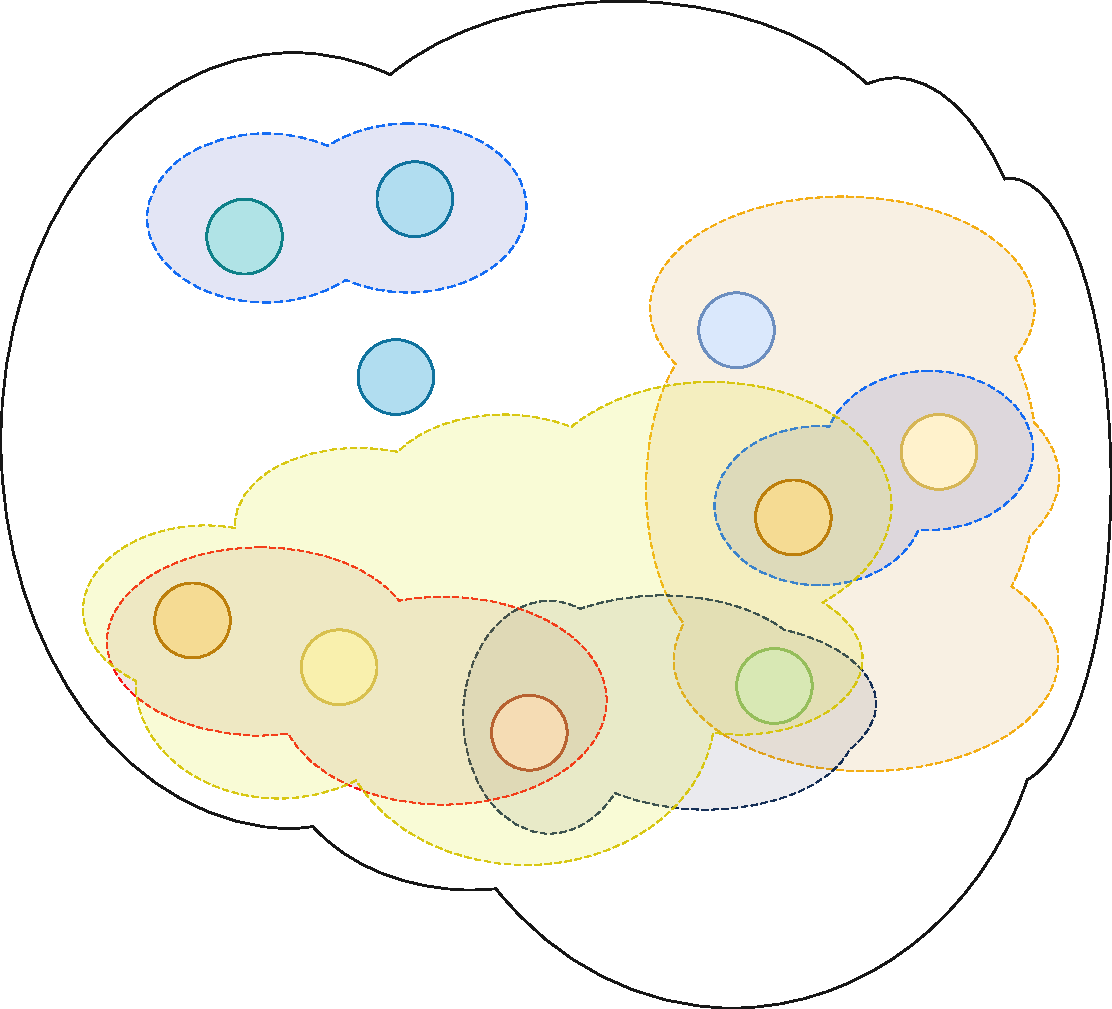
\includegraphics[width=0.6\textwidth]{figures/processes}
    \caption{
        Aggregate processes executed on a collective operating system.
        Solid circumferences represent devices, their internal color indicates the device kind
        (same color, same kind).
        The space delimited by the solid black line indicates the region of the space where the
        \ac{os} is active.
        Dashed zones are aggregate processes,
        the same color indicates the same process.
        Notice that devices may participate in one, none, or multiple processes.
        Also, differently than the current proposal for aggregate processes,
        with the proposed approaches the same process can be non-contiguous in space-time.
    }\label{fig:processes}
\end{figure}

The general idea of the project is conveyed graphically by
\Cref{fig:system} and \Cref{fig:processes}.
%
\Cref{fig:system} shows a high-level view of the system,
where the \ac{cos} works as middleware between the different aggregate programs and the devices where they run.
%
From another perspective,
\Cref{fig:processes} shows aggregate processes that execute over the shared \ac{os},
involving different sub-portions of the space-time.
%
Each process can be executed on different devices and a device can execute different processes,
so it is possible to have an overlap of processes on the devices.
%
Note that, differently than the current aggregate processes~\cite{EAAI2020-processes},
through the proposed approach the shared \ac{os} permits processes which are non-contiguous in space.

Differently from the \ac{dos},
the \ac{cos} is situated and can manage multiple aggregate processes executed on many devices,
with the aim of evaluating the processes as a collective distributed across space and time.

\subsection{Research goals and challenges}
\label{subsec:research-goals-and-challenges}

Realizing such a system requires an understanding of the meaning of various concepts when they are tied to space and time.

\paragraph{Users and permissions.}
\label{par:users-and-permissions}
In classic \acp{os} exists a subdivision of users and groups,
and access to resources and services is based on the user's role relative to the context in which they are located.
%
In an aggregate or collective context,
at the moment,
there is no clear definition if what a user (or group) is and how to manage its permissions inside the collective system.
%
For example,
in a crowd management scenario,
there are multiple types of users:
the people who are part of the crowd and the law enforcement officers who manage the crowd.
%
Clearly,
the law enforcement officers have more permissions than the people in the crowd and can execute different actions.

\paragraph{Signals and interrupts.}
\label{par:signals-and-interrupts}
Similarly, the concept of interrupt and signal cannot be simply inherited from the traditional \acp{os},
and needs rethinking.
%
Signals are a similar problem as permissions, it must be clear who sends a signal because it can
change the behavior of the recipient process.
%
It must be possible to send a signal (such as a termination or kill signal) to an aggregate process specifically,
without affecting the others;
moreover,
not every user in the system can send arbitrary signals to arbitrary aggregate processes:
in this sense,
the management of signals is tightly coupled with the capability of managing permissions in space and time.
%
Moreover,
it must be investigated what a pause or continue or kill signal means in an aggregate environment.
%
For instance,
in the aggregate processes approach termination is managed collectively and cannot be interrupted yet. %todo check
%
However,
there may be situations where a single device decides to terminate processes or where a process using shared
resources loses the right to use them during execution,
introducing a distributed consensus problem.

Using the example of the crowd management scenario,
there may be situations involving crowd sensing or crowd steering where law enforcement realizes that too many people are gathering.
%
Depending on the situation,
third-party entities allowed to send certain kinds of signals can decide to interrupt the crowd-management process.

The necessity of sending signals to processes while they are running establishes the need for a mechanism to enable changes to the system's behavior at runtime.

\paragraph{Intra-process communication.}
\label{par:intra-process-communication}
Communication between processes in different regions of space is another issue that needs to be addressed.
%
For example,
in a crowd steering and crowd tracking scenario,
there are different processes that need to communicate between them to manage the crowd.
%
A process managing the crowd steering needs to communicate with the process that is managing the crowd tracking,
to understand where the people are and how to move them.

Moreover, intra-process communication,
mediated by shared memory spaces or files in traditional systems,
is not applicable as-is when processes are inherently distributed,
so further research is needed from this point of view.
%
Actually,
this feature is not present in the current aggregate processes,
where the communication between processes is not allowed. %todo check

\paragraph{Distributed sensors and actuators.}
\label{par:distributed-sensors-and-actuators}
Another challenge is the management of distributed sensors and actuators.
%
Combining the capabilities of multiple devices to achieve a common observation as a single entity or logical resource,
can lead to a more abstract and high-level programming approach,
and to involve heterogeneous devices in the system,
seen as a ``collective sensor'',
realizing a form of ``sensor fusion''~\cite{sasiadek2002sensor} at the application level.
%
In the crowd management scenario,
various sensors or devices may be involved in observing the crowd and sending data to the system for management.
%
The system should treat data received from different devices as if it were from a single entity,
allowing for a more abstract and high-level programming approach.
\\

The proposed research project therefore aims to investigate the development of \emph{\ac{cos}},
based on the \ac{ac} paradigm.
%
The paradigm itself of \ac{ac} also offers consistency and resilience to failures,
and the possibility to adapt to \emph{dynamic} changes in the environment.

\subsection{Reference scenarios}
\label{subsec:example-applications}

\sloppypar
\paragraph{Crowd management.}
The system can find application in various scenarios,
such as the crowd management or surveillance scenario.
%
The system can be applied to manage the movement of the people to avoid congestion,
by sensing the crowd and steering it in a certain direction to prevent overcrowding and dangerous situations.
%
In this case,
there may be several drones, or sensors, who are running the same aggregate process,
observing the crowd and sending data to the system,
which sees them as a single entity (distributed sensors and actuators).
%
People in the crowd are managed by evaluating the data received,
letting another process direct the movement of the people.
%
As previously discussed,
the two processes need to communicate between them to manage the crowd in an efficient way (intra-process communication),
making people move in the right direction depending on the situation.
%
There may also be a need for law enforcement intervention to manage the crowd (users and permissions),
sending signals or interrupts to the processes in execution to change the direction of the crowd.

\sloppypar
\paragraph{Autonomous navigation.}
One of the problems presented in the aforementioned collaboration with prof. Sven Tomforde,
involves communication between maritime autonomous surface ships in the Kiel Canal.
%
Ships use different technologies to communicate with each other,
depending on the distance between them,
with data rates extremely different depending on the technology used.
%
Specifically,
the farther apart the ships are,
the fewer data they can exchange due to the technology of communication available;
for instance,
the ships in a shorter range typically communicate through 5G and can exchange more data between them,
rather than the ships in a longer range that send data using satellite communication.
%
It is believed that through \ac{ac},
and particularly through the use of \ac{xc},
a contribution can be made towards solving this problem.
%
The system should automatically adapt to the appropriate technology of communication,
choosing the priority data to exchange between the ships,
therefore minimizing the errors in the communication between them.

\sloppypar
\paragraph{Light management in a smart city.}
Many other application scenarios can be considered,
such as avoiding light pollution or traffic congestion in a smart city.
%
It could also be useful to manage the city's lighting based on the presence of people in the streets to avoid light pollution and save energy,
or to manage the traffic lights based on the presence of cars in the streets to avoid traffic congestion.

% ----------------------------------------
\section{Expected results}
\label{sec:expected-results}

As results of the proposed research project,
it is expected to bring
\begin{inlinelist}
    \item a contribution to the advancement of scientific and technological knowledge in the field of \ac{ac} and \ac{cas},
    \item a theoretical and executable model of the \ac{cos},
    \item a prototype of the system that is able to manage scenarios at least in a simulated environment,
    taking as reference scenarios the crowd management and the autonomous navigation scenarios mentioned in \Cref{subsec:example-applications}.
\end{inlinelist}

As a long-term vision,
the system will be able to manage many devices in a collective environment,
where the devices can be heterogeneous and can change over time.
%
Some of the application scenarios where the system can be used are
\begin{inlinelist}
    \item \emph{smart cities},
    \item \emph{swarm scenarios},
    \item \emph{crowd management},
    \item \emph{morphogenesis},
    \item \emph{autonomous vehicles},
    \item \emph{surveillance}.
\end{inlinelist}

% ----------------------------------------
\section{Subdivision of the project and timeline}
\label{sec:subdivision-of-the-project-and-timeline}

\begin{figure}
    \centering
    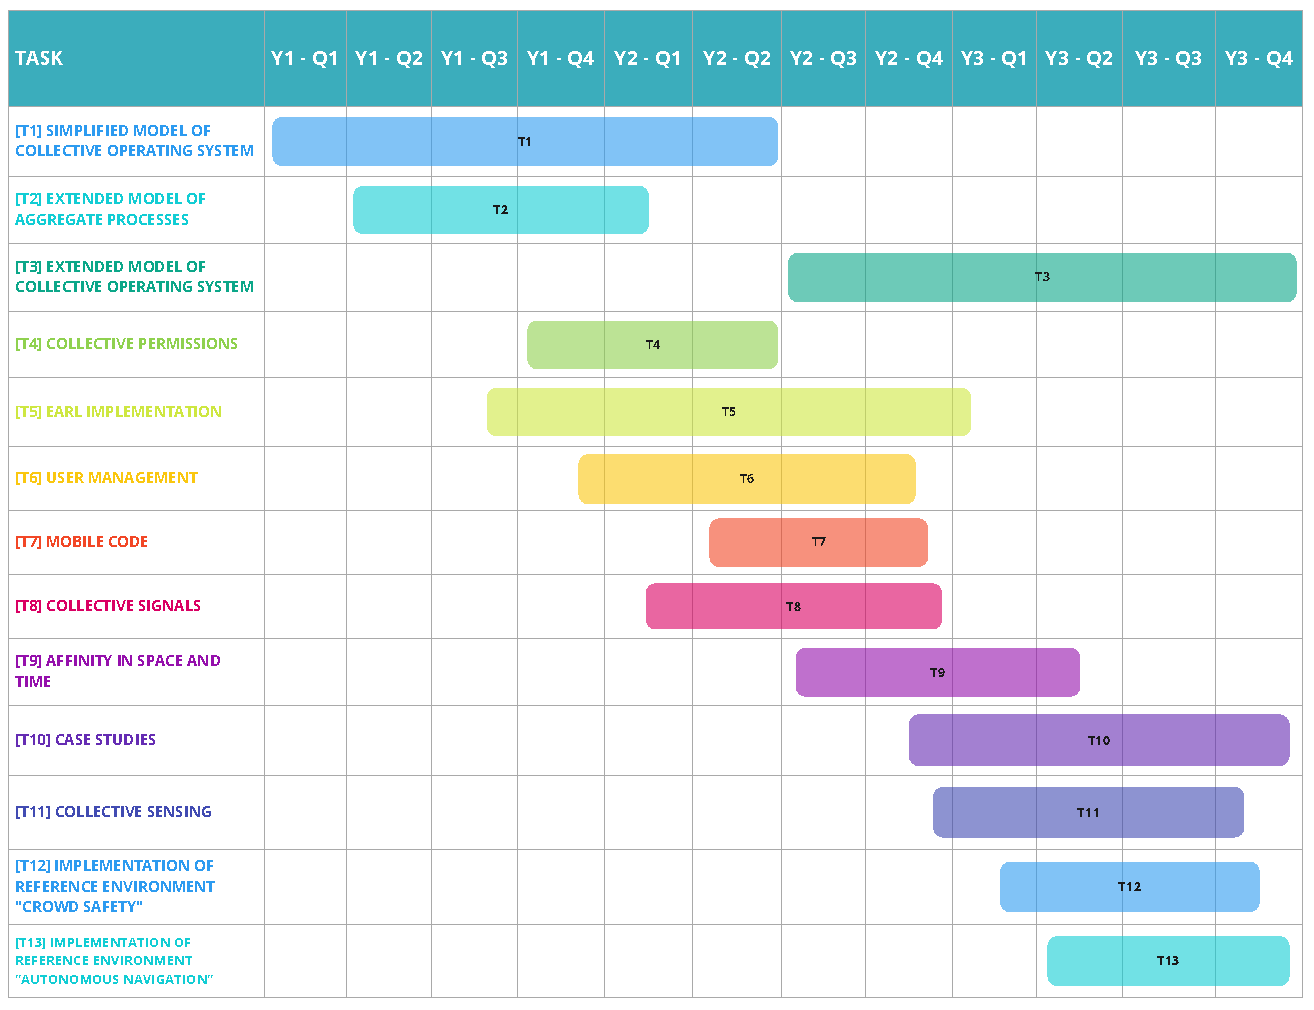
\includegraphics[width=0.99\textwidth]{figures/timeline}
    \caption{Hypothetical timeline of the three-year project.
        Years are subdivided in quarters, Q1 is from January to March,
        Q2 is from April to June, Q3 is from July to September, and Q4 is from October to December.
    }\label{fig:timeline}
\end{figure}

In the \Cref{fig:timeline} is shown a hypothetical timeline with tasks of the three years of the project,
where each year is subdivided into quarters.

\sloppypar
\paragraph{First year}
In the first year of the project,
it is essential to thoroughly investigate the state of the art and create a simplified model of how the new system should work.
%
The simplified model will include the definition of the main interconnected concepts of the system,
such as the implementation of the aggregate processes,
the management of permissions and the collective sensing of external devices.
%
Following this,
the actual development process begins with the prototype implementation in the target language Collektive.
%
At the end of the first year,
there will be enough foundations to start the development of the system in a use case scenario.
%
The use case will be relevant to the crowd safety scenario,
including crowd steering, sensing, and tracking.

\sloppypar
\paragraph{Second year}
The second year of the project will be focused on completing the simplified model of the system,
leading to the development of the extended model,
that includes the management of users or groups, signals and interrupts, and intra-process communication.
%
Throughout the year,
the focus will be on continuing the development of the prototype,
expanding on the concepts investigated in the first year,
and incorporating features such as runtime aggregate programs injection.
%
Eventually,
when considering the international research stay,
the plan is to establish contacts with companies or research groups that possess the necessary hardware to test the system.
%
Towards the end of this period,
the first use case will be implemented and tested in a simulated environment,
leaving space to the implementation of the second use case inherent to the autonomous navigation scenario.

\sloppypar
\paragraph{Third year}
In the third and final year of the project,
the extended model of the system will be completed, alongside the development of the prototype
and the implementation of the third use case scenario mentioned before.

% ----------------------------------------
\section{Proposed evaluation criteria}
\label{sec:proposed-evaluation-criteria}

\sloppypar
\paragraph{Qualitative.}
Qualitative evaluation will be based on the development of open-source software capable of being used in simulations and real-world
environments on heterogeneous devices.
%
The degree of success will depend on the features implemented among those previously discussed.

\sloppypar
\paragraph{Quantitative.}
Experiments will be conducted at least in a simulated environment,
eventually in a real-world scenario with the help of a partnership where appropriate hardware is available.
%
Therefore,
metrics to evaluate the system will be defined depending on the use case scenario;
will be then compared with the state-of-the-art approaches and with an oracle system,
to understand how far from the optimal solution the system is.

However,
as field-testing is more challenging due to the need for specific hardware.
the possibility of securing a partnership for an international research stay during the PhD program will be pursued,
where appropriate hardware is available to test the project.
%
%\sloppypar
%\paragraph{Scientific contribution.}
%In terms of scientific results and dissemination,
%the goal is to produce and submit papers to approximately one or two conferences per year and to have a couple of articles submitted to journals.
%%
%The focus will be on the key communities, which have as topic ``self-organizing systems'',
%such as \emph{ACSOS}\footnote{\url{https://acsos.github.io}} or \emph{SEAMS}\footnote{\url{https://conf.researchr.org/home/seams-2025}},
%or even journals such as \emph{ACM TAAS}\footnote{\url{https://dl.acm.org/journal/taas}}.
%
%\sloppypar
%\paragraph{Dissemination.}
%Another way to evaluate the success of the project is through the creation of international collaborations.
%%
%Several experts have already been identified,
%particularly prof. Sven Tomforde,
%who has expressed interest in collaborating.
%%
%Additionally,
%I hope to discuss potential collaborations soon with a network of experts who have participated in the aforementioned conferences,
%such as prof. Lukas Esterle and prof. Alessandro Papadopoulos,
%who have already worked with our research group.

% ----------------------------------------
\bibliographystyle{IEEEtran}
\bibliography{bibliography}

\end{document}
